%%%%%%%%%%%%%%%%%%%%%%%%%%%%%%%%%%%%%%%%%%%%%%%%%%%%%%%%%%%%%%%%%%%%%%%%%%%%%%%%%%%%%%%%%%%%%%%%%%%%%%%%%%%%%%%%%%%%%%%%%%%%%%%%%%%%%%%%%%%%%%%%%%%%%%%%%%%%%%%%%%%%%%%%%%%%%%%%%%%%%%%%%%%%%%%%%%%%%%%%%%%%%%%%%%%%%%%%%%%%%%%%%%%
%%%%%%%%%%%%%%%%%%%%%%%%%%%%%%%%%%%%%%%%%%%%%%%%%%%%%%%%%%%%%%%%%%%%%%%%%%%%%%%%%%%%%%%%%%%%%%%%%%%%%%%%%%%%%%%%%%%%%%%%%%%%%%%%%%%%%%%%%%%%%%%%%%%%%%%%%%%%%%%%%%%%%%%%%%%%%%%%%%%%%%%%%%%%%%%%%%%%%%%%%%%%%%%%%%%%%%%%%%%%%%%%%%%
%%%%%%%%%%%%%%%%%%%%%%%%%%%%%%%%%%%%%%%%%%%%%%%%%%%%%%%%%%%%%%%%%%%%%%%%%%%%%%%%%%%%%%%%%%%%%%%%%%%%%%%%%%%%%%%%%%%%%%%%%%%%%%%%%%%%%%%%%%%%%%%%%%%%%%%%%%%%%%%%%%%%%%%%%%%%%%%%%%%%%%%%%%%%%%%%%%%%%%%%%%%%%%%%%%%%%%%%%%%%%%%%%%%
\chapter{The Large Hadron Collider}

The Large Hadron Collider (LHC)~\cite{bib:LHC_machine_2008,bib:LHC_2004} is a particle accelerator installed in the former LEP~\cite{bib:LEP_design_1984} tunnel at CERN~\cite{bib:CERN:web}.
It is 26.7~\km in circumference and consists out of two separate rings, which are, in periods of operation, inhabited by two counter-circulating beams.
At the interaction points of the two beams, either proton-proton collisions or heavy ion collisions take place.
In this thesis, only collision data from the year 2012 is analysed.
Thus all machine values cited in the following chapters and paragraphs refer to the setup in 2012 (if not stated otherwise).

The beams are separated into bunches which rotate with a bunch spacing of 50\ns corresponding to a collision frequency of 20\mhz.
Before the bunches are actually filled into the LHC rings they are pre-accelerated in other accelerators, which are (in the order they are actually passed by the protons) Linac2, Proton  Synchrotron Booster (PSB), Proton Synchrotron (PS), Super Proton Synchrotron (SPS).
The injector chain and the LHC ring with its experiments is visualised in Fig~\ref{fig:LHC}.
\begin{figure}[!b]
  \centering
      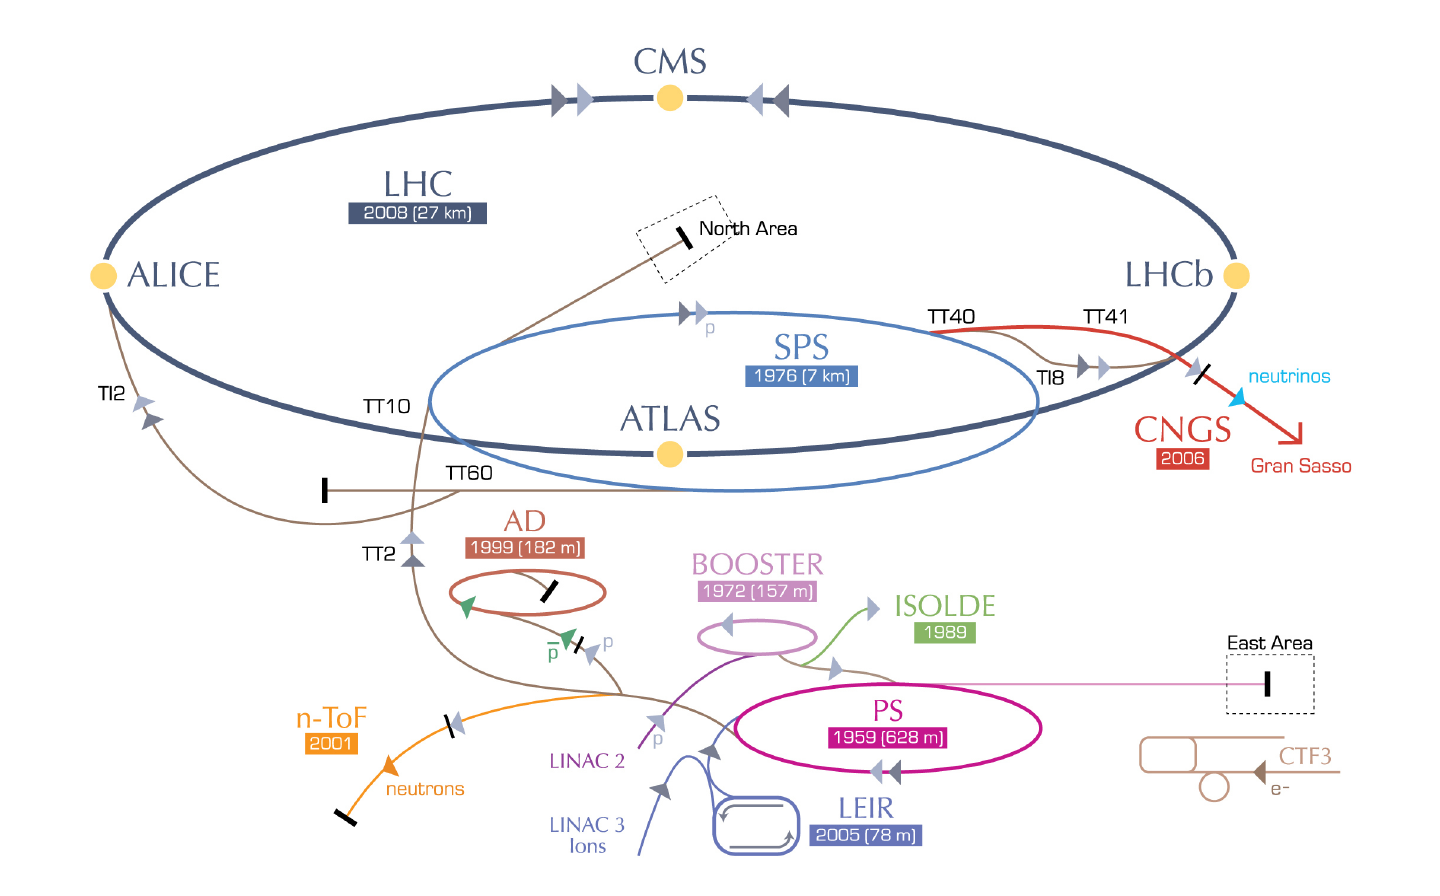
\includegraphics[width=0.79\textwidth]{figures/experiment/LHC/LHC_small.png}
  \caption{Visualisation of the LHC with its experiments and the injector chain. Taken from~\cite{bib:CERNBrochure}.}  
  \label{fig:LHC}
\end{figure}

In the LHC, the beams are kept on the circuit with the help of a magnetic field of 4.76\tesla.
Further quadrupole and sextupole magnets squeeze and focus the bunches.
They have a spread of roughly 8\cm length and a Gaussian shape radius of 20\mum RMS at the interaction point.
The number of contained protons in each bunch is of the order $10^{11}$.
The LHC has eight different insertion region, where four of them are dedicated to the four main experiments of the LHC, the CMS, ATLAS, LHCb and ALICE experiments.
The CMS~\cite{bib:CMS:experiment,bib:CMS:TDR} and ATLAS~\cite{bib:ATLAS:experiment,bib:ATLAS:TDR_1,bib:ATLAS:TDR_2} experiments are so-called ``general purpose experiments'', not designed for one specific task.
In contrary, the LHCb~\cite{bib:LHCb:experiment} and the ALICE~\cite{bib:ALICE:experiment} experiment are designed with an emphasis on CP-violation measurements and heavy ion collisions, respectively.
Each experiment is interested thus in different processes to happen at the beam collision points.
The number of expected event for a given process can be expressed in terms of the corresponding cross section $\sigma$ times the integrated luminosity.
\begin{equation}
N = L \cdot \sigma,
\end{equation}
with an integrated luminosity of $L=\int \mathcal{L}\, dt$, where $\mathcal{L}$ is the instantaneous luminosity (which can change over time).

The instantaneous luminosity $\mathcal{L}$ depends on the several machine parameters, such as the collision frequency $f$, the number of particles in the bunches $n_1$ and $n_2$,
the spread in the transverse plane of the bunches $\sigma_x$ and $\sigma_y$ and a geometrical correction parameter $F$ due to the crossing angle of the two bunches at the interaction point
\begin{equation}
\mathcal{L} = \frac{f n_1 n_2 }{4 \pi \sigma_x \sigma_y} \cdot F.
\end{equation}
In 2012, the peak luminosity was $7.7 \cdot 10^{33} \frac{1}{\text{cm}^2\,\text{s}}$.
The total integrated luminosity over time recorded at the CMS experiment is shown in Fig.~\ref{fig:Lumi}.

\begin{figure}[!b]
  \centering
      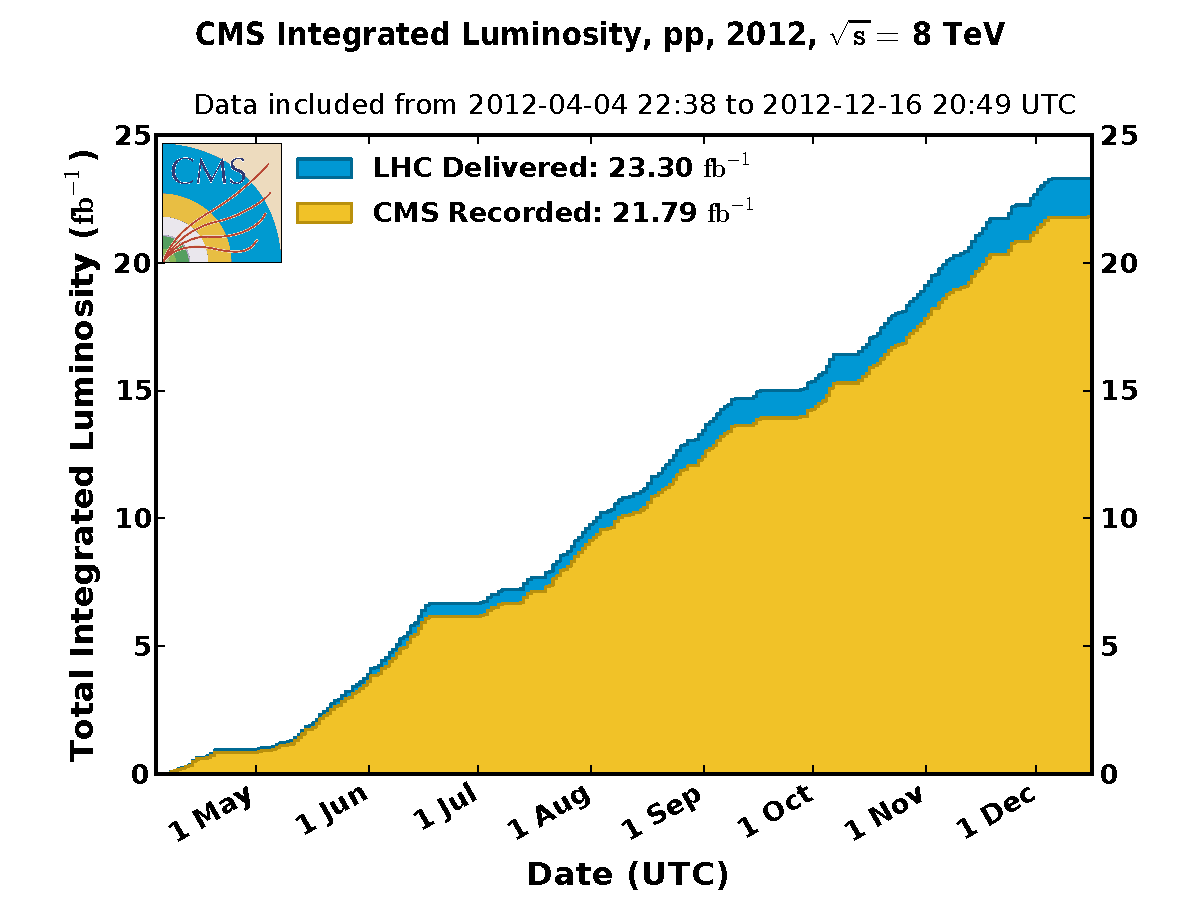
\includegraphics[width=0.59\textwidth]{figures/experiment/LHC/int_lumi_per_day_cumulative_pp_2012.pdf}
  \caption{Integrated luminosity delivered by LHC (blue) and recorded by CMS (orange) in the year 2012. Taken from~\cite{bib:LumiWiki}.}  
  \label{fig:Lumi}
\end{figure}

%%%%%%%%%%%%%%%%%%%%%%%%%%%%%%%%%%%%%%%%%%%%%%%%%%%%%%%%%%%%%%%%%%%%%%%%%%%%%%%%%%%%%%%%%%%%%%%%%%%%%%%%%%%%%%%%%%%%%%%%%%%%%%%%%%%%%%%%%%%%%%%%%%%%%%%%%%%%%%%%%%%%%%%%%%%%%%%%%%%%%%%%%%%%%%%%%%%%%%%%%%%%%%%%%%%%%%%%%%%%%%%%%%%
%%%%%%%%%%%%%%%%%%%%%%%%%%%%%%%%%%%%%%%%%%%%%%%%%%%%%%%%%%%%%%%%%%%%%%%%%%%%%%%%%%%%%%%%%%%%%%%%%%%%%%%%%%%%%%%%%%%%%%%%%%%%%%%%%%%%%%%%%%%%%%%%%%%%%%%%%%%%%%%%%%%%%%%%%%%%%%%%%%%%%%%%%%%%%%%%%%%%%%%%%%%%%%%%%%%%%%%%%%%%%%%%%%%
%%%%%%%%%%%%%%%%%%%%%%%%%%%%%%%%%%%%%%%%%%%%%%%%%%%%%%%%%%%%%%%%%%%%%%%%%%%%%%%%%%%%%%%%%%%%%%%%%%%%%%%%%%%%%%%%%%%%%%%%%%%%%%%%%%%%%%%%%%%%%%%%%%%%%%%%%%%%%%%%%%%%%%%%%%%%%%%%%%%%%%%%%%%%%%%%%%%%%%%%%%%%%%%%%%%%%%%%%%%%%%%%%%%
\FloatBarrier
\chapter{CMS detector}
The Compact Muon Solenoid (CMS) detector~\cite{bib:CMS:experiment,bib:CMS:TDR} is a general purpose detector, designed to explore particle physics phenomena up to the multi-TeV scale.
The detector concept is an onion-like structure of different layers, each one made up with a different type of detector.
In Fig.~\ref{fig:CMSdetector}, a perspective view of the CMS detector is depicted. 
\begin{figure}[!b]
  \centering
      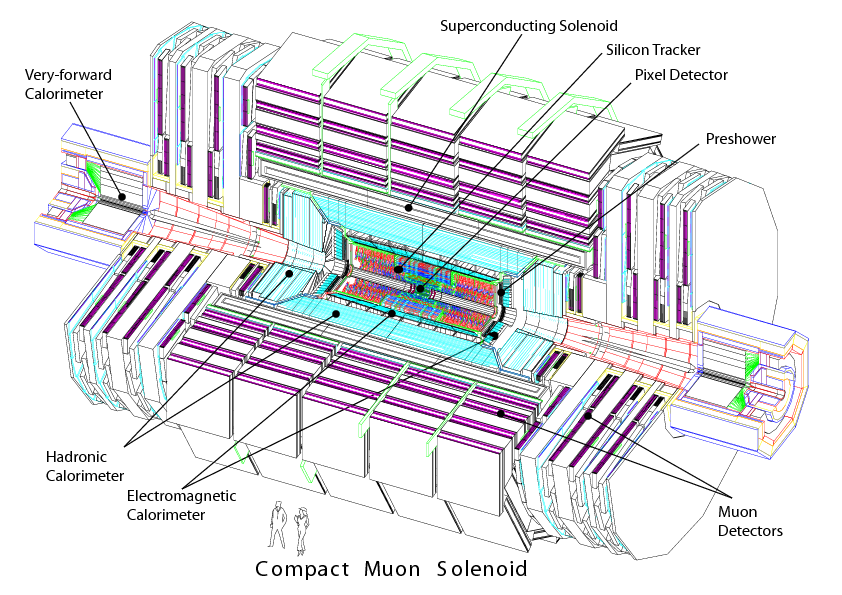
\includegraphics[width=0.99\textwidth]{figures/experiment/CMS/cms_complete_labelled.png}
  \caption{A perspective view of the CMS detector. Taken from~\cite{bib:CMS:experiment}}  
  \label{fig:CMSdetector}
\end{figure}
The used coordinate system at the CMS experiment consists of the pseudorapidity $\eta = -\ln \tan{\frac{\theta}{2}}$ and the azimuthal angle $\phi$.
The advantage of the pseudorapidity $\eta$ is the Lorentz invariance with respect to the z-axis (beam axis).
The angle $\phi$ covers the direction in the $x-y$ plane (orthogonal to the beam axis).

In the following, the various detector components of the CMS detector from the inside to the outside will be explained.
In order to ensure a possible measurement in the first detector component, a magnetic field is needed in order to bend the particles' trajectories.
At the CMS experiment, this magnet is lcoated between the hadron calorimeetr and the muon chmabers.
it is vxxx return yokes and further bla.


%%%%%%%%%%%%%%%%%%%%%%%%%%%%%%%%%%%%%%%%%%%%%%%%%%%%%%%%%%%%%%%%%%%%%%%%%%%%%%%%%%%%%%%%%%%%%%%%%%%%%%%%%%%%%%%%%%%%%%%%%%%%%%%%%%%%%%%%%%%%%%%%%%%%%%%%%%%%%%%%%%%%%%%%%%%%%%%%%%%%%%%%%%%%%%%%%%%%%%%%%%%%%%%%%%%%%%%%%%%%%%%%%%%
\FloatBarrier
\section{The tracking system}

The tracking detector~\cite{bib:CMS:Tracker_1997,bib:CMS:Tracker_2000} is the innermost detector of the CMS experiment. 
It is a silicon semiconductor detector and is included for the tasks of vertex and track reconstruction by the measurement of particle's energy losses.
Additionally, the energy measurements can be used for measuring a particle's \dedx.
A schematic sketch of the tracker at CMS is depicted in Fig.~\ref{fig:Tracker}.
\begin{figure}[!b]
  \centering
      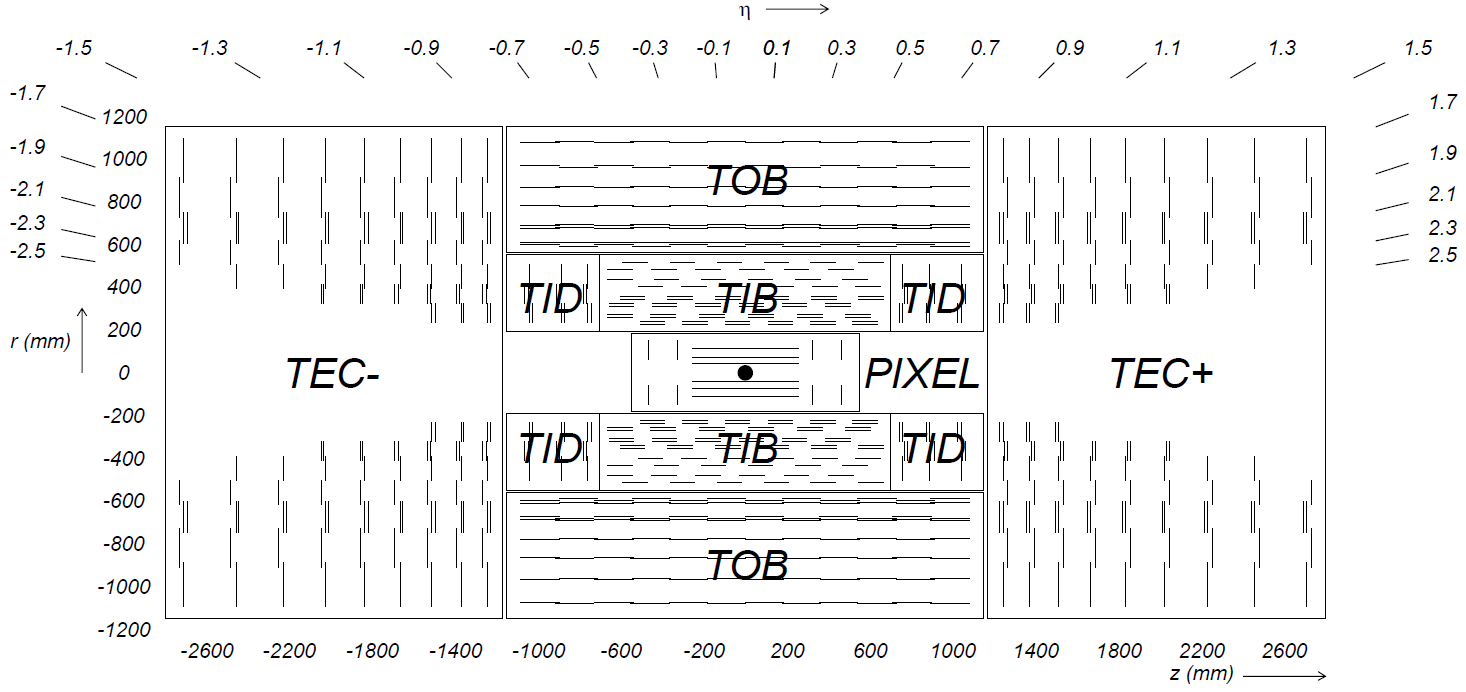
\includegraphics[width=0.99\textwidth]{figures/experiment/CMS/Figures_Experimental_Apparatus_Tracker.png}
  \caption{Schematic sketch of the silicon tracker at CMS in the $z - \phi$ plane. Taken from~\cite{bib:CMS:tracking_8TeV}.}  
  \label{fig:Tracker}
\end{figure}
The tracking system is devided into parts using different technologies. First, a silicon pixel detector and second, a silicon strip detector.
How both are constructed, will be explained in the following two sections.
As a calibration of the silicon pixel detector was performed within this PhD thesis (see Section~\ref{sec:EnergyCalibration}), an emphasis will be put on the pixel detector.

%%%%%%%%%%%%%%%%%%%%%%%%%%%%%%%%%%%%%%%%%%%%%%%%%%%%%%%%%%%%%%%%%%%%%%%%%%%%%%%%%%%%%%%%%%%%%%%%%%%%%%%%%%%%%%%%%%%%%%%%%%%%%%%%%%%%%%%%%%%%%%%%%%%%%%%%%%%%%%%%%%%%%%%%%%%%%%%%%%%%%%%%%%%%%%%%%%%%%%%%%%%%%%%%%%%%%%%%%%%%%%%%%%%
\subsection*{The silicon pixel tracker}
The silicon pixel detector consists of three different cylindrical layers in the barrel region (at radii of 4.4\cm, 7.3\cm and 10.2\cm) and two discs in the encaps (at $z$-distances of 34.5\cm and 46.5\cm) (cf. Fig.~\ref{fig:Tracker}).
It is made up of 1440 modules in total (barrel + endcap), each module containing 8 or 16 read-out-chips (ROCs).
Each read-out-chip is bumb bonded~\cite{FIXME} to a pixel system of $52\times80$ pixels, that are read out in double columns.
A visualisation of the pixel system is shown in Fig.~\ref{fig:PixelTracker}.
\begin{figure}[!t]
  \centering
      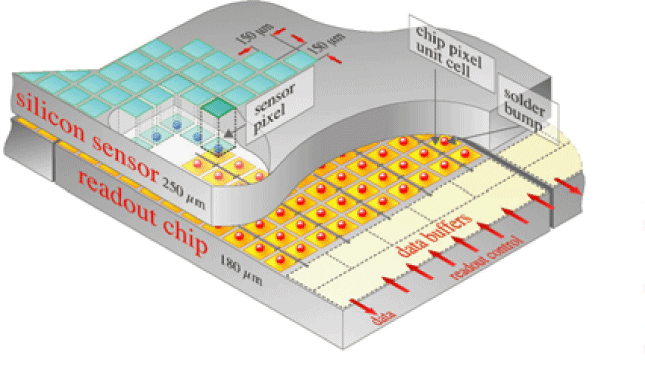
\includegraphics[width=0.99\textwidth]{figures/experiment/CMS/Pixelement.png}
  \caption{Schematic sketch of a part of a silicon pixel tracker module icnluding the silicon sensors and the read-out-chip (ROC). Taken from~\cite{bib:CMS:tracking_8TeV}.}  
  \label{fig:PixelTracker}
\end{figure}

The silicon pixel detector is very important for the reconstruction of primary and secondary vertices as well as the reconstruction of particles' tracks.
Therefore a high spatial resolution is needed.
This is achieved by the small size of the pixels ($ 150 \times 100 \mum^2$) and the exploitation of the spread of the energy deposition across several pixels (in average the energy is deposited across 2-4 pixels FIXME).
% By the measurement of the spread of the deposited energies accross several pixels, a so-called cenetr-of gravity can be determined making the spactial resolution much better than the pixel size.
Exploting this spread across pixels, a spatial resolution of $13\times14\mum^2$ in the barrel region and $10\times17\mum^2$ in the encaps can be achieved~\cite{FIXME}. 
The high spatial resolution makes the pixel detector perfectly suited for the reconstruction of vertices.

\subsection*{The silicon strip tracker}
The silicon strip tracker is the next to innermost detector of the CMS experiment.
It is devided into strips

\subsection*{Energy measurements in the tracking system}

\section{The calorimeters}
\subsection*{The electromagnet calorimeter}
\subsection*{The Hadronic calorimeter}

\section{The muon system}

\section{The trigger system}

\begin{itemize}
\item General purpose detector (picture) - short overview (tarcker, calorimeters, etc), pseudorapittyt and phi and z
\item Tracker (Pixel tracker - silicon strip tracker - energy measurements in the tracker )
\item Calorimeter - eCAL and HCAL
\item Muon system
\item Trigger system
\item 10 pages
\end{itemize}

%%%%%%%%%%%%%%%%%%%%%%%%%%%%%%%%%%%%%%%%%%%%%%%%%%%%%%%%%%%%%%%%%%%%%%%%%%%%%%%%%%%%%%%%%%%%%%%%%%%%%%%%%%%%%%%%%%%%%%%%%%%%%%%%%%%%%%%%%%%%%%%%%%%%%%%%%%%%%%%%%%%%%%%%%%%%%%%%%%%%%%%%%%%%%%%%%%%%%%%%%%%%%%%%%%%%%%%%%%%%%%%%%%%
%%%%%%%%%%%%%%%%%%%%%%%%%%%%%%%%%%%%%%%%%%%%%%%%%%%%%%%%%%%%%%%%%%%%%%%%%%%%%%%%%%%%%%%%%%%%%%%%%%%%%%%%%%%%%%%%%%%%%%%%%%%%%%%%%%%%%%%%%%%%%%%%%%%%%%%%%%%%%%%%%%%%%%%%%%%%%%%%%%%%%%%%%%%%%%%%%%%%%%%%%%%%%%%%%%%%%%%%%%%%%%%%%%%
%%%%%%%%%%%%%%%%%%%%%%%%%%%%%%%%%%%%%%%%%%%%%%%%%%%%%%%%%%%%%%%%%%%%%%%%%%%%%%%%%%%%%%%%%%%%%%%%%%%%%%%%%%%%%%%%%%%%%%%%%%%%%%%%%%%%%%%%%%%%%%%%%%%%%%%%%%%%%%%%%%%%%%%%%%%%%%%%%%%%%%%%%%%%%%%%%%%%%%%%%%%%%%%%%%%%%%%%%%%%%%%%%%%
\FloatBarrier
\chapter{Event reconstruction and particle identification}

Event reconstruction relies on very complicated algorthms bla


%%%%%%%%%%%%%%%%%%%%%%%%%%%%%%%%%%%%%%%%%%%%%%%%%%%%%%%%%%%%%%%%%%%%%%%%%%%%%%%%%%%%%%%%%%%%%%%%%%%%%%%%%%%%%%%%%%%%%%%%%%%%%%%%%%%%%%%%%%%%%%%%%%%%%%%%%%%%%%%%%%%%%%%%%%%%%%%%%%%%%%%%%%%%%%%%%%%%%%%%%%%%%%%%%%%%%%%%%%%%%%%%%%%
%%%%%%%%%%%%%%%%%%%%%%%%%%%%%%%%%%%%%%%%%%%%%%%%%%%%%%%%%%%%%%%%%%%%%%%%%%%%%%%%%%%%%%%%%%%%%%%%%%%%%%%%%%%%%%%%%%%%%%%%%%%%%%%%%%%%%%%%%%%%%%%%%%%%%%%%%%%%%%%%%%%%%%%%%%%%%%%%%%%%%%%%%%%%%%%%%%%%%%%%%%%%%%%%%%%%%%%%%%%%%%%%%%%
%%%%%%%%%%%%%%%%%%%%%%%%%%%%%%%%%%%%%%%%%%%%%%%%%%%%%%%%%%%%%%%%%%%%%%%%%%%%%%%%%%%%%%%%%%%%%%%%%%%%%%%%%%%%%%%%%%%%%%%%%%%%%%%%%%%%%%%%%%%%%%%%%%%%%%%%%%%%%%%%%%%%%%%%%%%%%%%%%%%%%%%%%%%%%%%%%%%%%%%%%%%%%%%%%%%%%%%%%%%%%%%%%%%
\FloatBarrier
\chapter{Event simulation}
